\documentclass[11pt,a4paper,oneside]{article}
\usepackage[latin1]{inputenc}
\usepackage{amsmath}
\usepackage{amsfonts}
\usepackage{amssymb}
\usepackage{graphicx}
\usepackage{color}
\usepackage {tikz}
\usepackage{fancyvrb}
\usepackage{caption}
\usepackage{subcaption}
\usepackage{float}
\usetikzlibrary {er}
\usepackage[left=2.00cm, right=2.00cm, top=1.00cm]{geometry}
\graphicspath{{./}}
\fvset{tabsize=4}

\begin{document}
	\title{DS 255 - System Virtualization \\ Assignment VI - High Level Language Virtual Machines}
	\author{Shriram R. \\ M Tech (CDS) \\ 06-02-01-10-51-18-1-15763}
	\maketitle	
	
	\begin{enumerate}
		\item Conventional Process VMs work on conventional ISAs which are not designed for portability or virtualization. Therefore, creating a high performance emulator is difficult. Also, emulating the OS interface exactly is challenging if the host and guest OS are different. All of this is because neither the guest nor the host platform is designed for virtualization.
		
		HLL VMs overcome this problem by building the application to a virtual-ISA whose primary design goal is portability. As shown below, HLL VMs are realized in the API Layer (2, 3 in the figure). The portable code which is in virtual-ISA is executed through a HLL VM interpreter/translator. Applications are not compiled for a specific OS. Rather, a set of standard API libraries is provided by the HLL environment to interact with the host OS for system calls.
		
		\begin{center}
			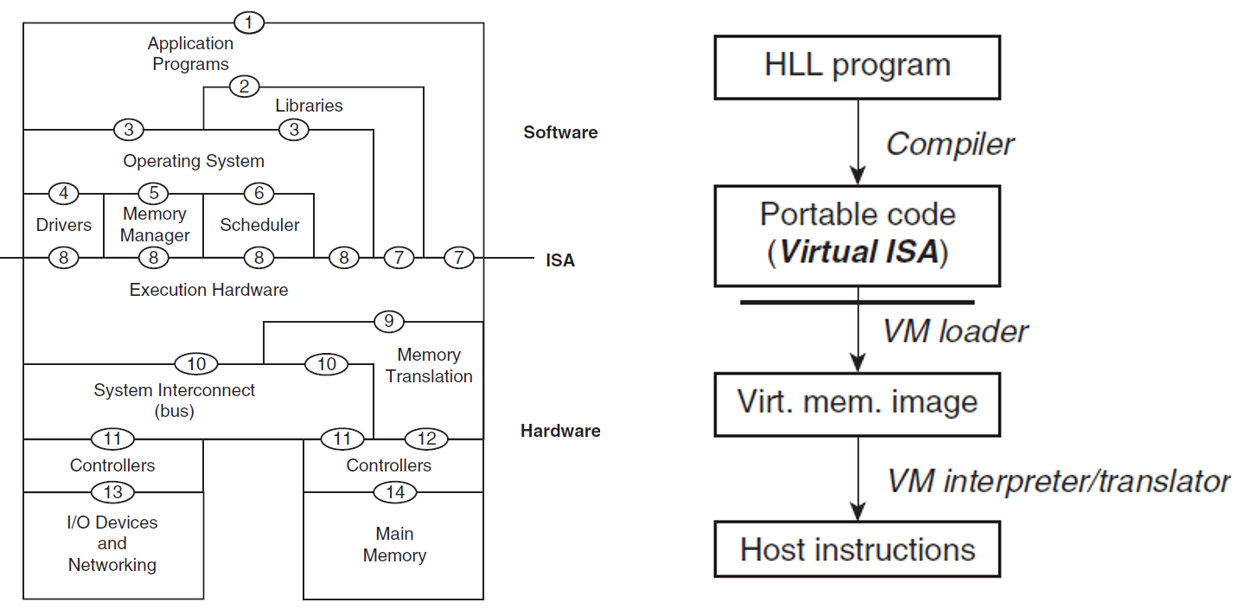
\includegraphics[scale=0.7]{4.png}
		\end{center}
		
		\item HLL VMs build generally upon virtual-ISA having instruction definitions (bytecodes) and data definitions (metadata). The major differences compared to conventional ISAs are as follows,
		\begin{enumerate}
			\item Virtual-ISAs consist of indefinite size memory model and memory addresses are invisible as opposed to fixed-size address space in conventional ISAs.
			\item Pointer arithmetic operations are generally not permitted and memory access is allowed only through explicit memory pointers with type checking employed.
			\item Operations are stack oriented which is agnostic to no. of registers in the hardware whereas conventional ISAs are register oriented.
			\item Indirect jumps are restricted in virtual-ISA and mixing of code and data is not permitted.
	    \end{enumerate}	
    
        \begin{verbatim}
                
        
        \end{verbatim}	
		
		\item The compatibility framework for JVM is defined by the JVM specification. Any implementation of JVM should adhere to this specification to ensure compatibility of java applications. The specification consists of following key components,
		\begin{enumerate}
			\item Data Types - Java consists of primitive data types like int, float etc. and references to objects. It also has objects and arrays which hold data in logical structures composed of primitive data types.
			\item Data Storage - Global, local and operand are three types of storage. All storage is divided into cells or slots which usually holds a single data item. All addressing is in terms of logical memory cells. Local and operand are allocated on stack and global is allocated on heap.
			\item Binary class - The combination of code and metadata is a binary class. Its format is the interface supported by the underlying VM. These classes can be loaded on demand. It consists of magic number for quick validation.
			\item Constant Pool - Constants can have variable length and can be shared. These are stored in a block known as constant pool. It is part of program's specification.
			\item Java instruction set - It is stack based and consists of specific instruction formats. It consists of data movement instructions, ALU instructions, type conversion, control flow instructions and specification for exceptions and errors.
		\end{enumerate}
		
		\item Stack architecture offer several merits which help in alleviating process virtual memory limits,
		\begin{enumerate}
			\item Stack architecture generally have undefined stack size which can be arbitrarily large. Even in the case of overflow, techniques like stack paging, demand fed single-element stack management, etc. can be used to handle it efficiently.
			\item Stack frames can be dynamically allocated for each method call with arguments, local storage and operand storage with different frames linked in a chain. 
			\item Stack based architecture makes fewer assumptions about target hardware (registers, address space limit etc.) thereby achieving the compatibility goal.
			\item The operands in a stack architecture are mostly implicit thereby reducing the size of object code significantly.
			\item It also enables faster operand access as it avoids operand fetching stage and can prefetch top operands from the top of the stack.
		\end{enumerate}
		
		\item The JVM memory layout consists of the following structure,
		      \begin{figure}[H]
		      	\centering
		      	\begin{subfigure}{.4\textwidth}
		      		\centering
		      		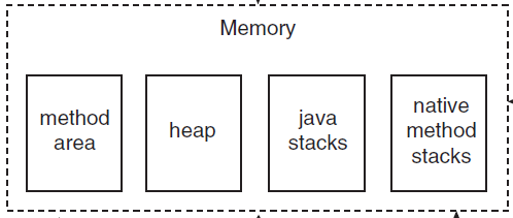
\includegraphics[scale=0.5]{1.png}
		      		\caption{Overview}
		      	\end{subfigure}%
		      	\begin{subfigure}{.4\textwidth}
		      		\centering
		      		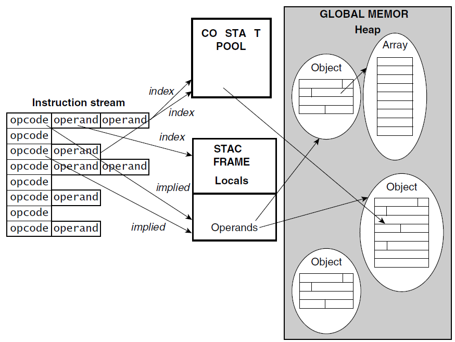
\includegraphics[scale=0.6]{2.png}
		      		\caption{Memory Hierarchy}
		      	\end{subfigure}		      	
		      \end{figure}
	      \begin{verbatim}
	      	      
	      \end{verbatim}
	      \begin{enumerate}
	      	\item Method area is implicitly defined as is used for holding the program instructions. This memory can be accessed only by the program counter (PC). It is never accessed by load and store instructions. PC cannot be inspected as well.
	      	\item Stack is used for local and operand storage. Procedure arguments are passed on the stack. A stack frame is allocated when a method is called. Exact size of the stack is not architected. StackOverFlow error is thrown if the size gets exceeded. A stack pointer cannot be explicitly inspected by a program. 
	      	\item Native stack is used for native methods that bind to java program through Java Native Interface (JNI). It is separate from java stack because these methods have their own stack specifications.
	      	\item The heap is used for dynamically allocated objects. It is of unspecified size. If heap runs out of space, OutOfMemoryError is thrown. A garbage collector can be used to reclaim heap memory when no longer needed by a program.
	      \end{enumerate}
      	  The memory hierarchy figure shows operands present in stack, arrays and objects present in heap, instruction stream and constant pool. 			
		
		\item The postfix notation for the expression: $100*2+5*(390+20/5)-(40-4*10)$ is given by, $$100\,\,2 * 5\,\,390\,\,20\,\,5\,\,/ + * + 40\,\,4\,\,10 * - -$$ The stack operations and contents are shown below, 
			  \begin{center}
			  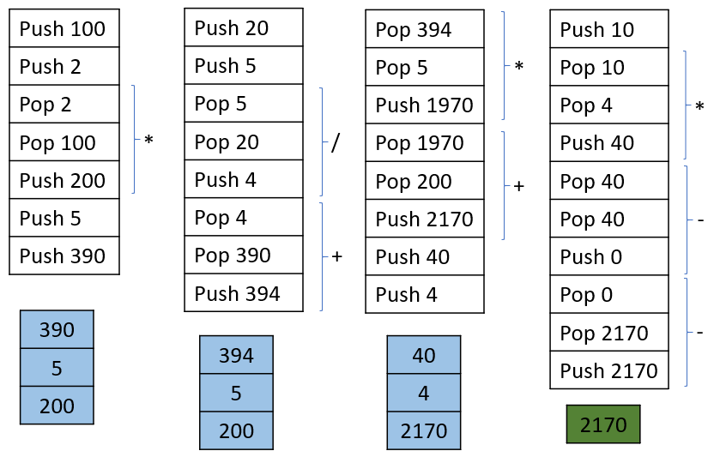
\includegraphics[scale=0.6]{3.png}
			  \end{center}
		 
		  
		\item Java security manager is needed for 1) protecting the VM software from the application 2) Preventing the guest application from accessing other files on both remote and local systems and 3) To strictly limit access to untrusted HLL programs within its domain. This means that HLL program can operate within its protection sandbox as managed code. The sandboxing model is supported by Java security manager as follows,
			  \begin{enumerate}
			    \item The security manager is a trusted class which is attached to a program during start to enforce user specified security policies related to file access, etc.
			    \item The security manager check method checks the requested operation to see if it is permitted and throws a security exception if it is not permitted. The checks will be in effect over the course of application runtime.
			    \begin{verbatim}
			    
			    
			    \end{verbatim}
			    \item The manager employs static and dynamic type checking to guard against read/write data in JVM's code and data memory solving one aspect of sandboxing.
			    \item It protects local and remote files through trusted java library (java.io API) whose methods check the security manager before invoking a OS call.
			  \end{enumerate}
			 The security manager can be customized to implement complex security policies. E.g. It can check if resource request is from remote method and control access accordingly through customization. 
		
		\item The concurrent garbage collectors have the following issues,
			  \begin{enumerate}
				\item The program might attempt to reference an object at the time when the pointers may be temporarily inconsistent causing synchronization issue.
				\item The program may be changing references at the time the collector is tracing a reference path leading to synchronization issue.
				\item During concurrent garbage collection, a partially collected heap may be in state of flux or unstable to be precise and require synchronization.
				\item An object which is marked might not be garbage collected if the pointer to marked object is changed before sweep process begins.
				\item Write barriers are provided for references to objects that are marked. When an already marked object is overwritten, the object pointed to is added to queue of marked objects.
			  \end{enumerate}
		
 		
%		\begin{center}
%			\begin{tabular}{|p{6.5cm}|p{6.5cm}|}
%				\hline 
%				\textbf{Advantages}  & \textbf{Disadvantages} \\
%				\hline
%				\end{tabular}
%		\end{center}   	
	        			
	\end{enumerate}
    
    \textbf{References}
    \begin{enumerate}
    	\item Jim Smith and Ravi Nair - Virtual Machines: Versatile Platforms for Systems and Processes  	
    	\item Course lecture notes
    \end{enumerate}
 

    
\end{document}